\documentclass{article}
\usepackage{pgfplots}
\pgfplotsset{compat=newest}

\pagestyle{empty}

\begin{document}
In this note we explore the problem of finding the maximum subarray sum in a randomly generated sequence of a given
length.

\section{Problem Statement}
The \textit{maximum subarray sum} of a given one-dimensional array of numbers that is randomly generated. The problem is to find the contiguous subarray within the array that has the largest sum.

\section{Experiment Setup}

For each problem size $N$, we create an array of size $N$ and initialize its values. The values are generated within the range $[-\frac{N}{3}, \frac{2N}{3}]$. For each $N$, we performed 1,000,000 experiments. The blue graph below shows the maximum value of maximum subarray sum. The red graph shows function $0.17x^2$ which grows almost at the same rate, supporting the hypothesis that maximum sum of the maximum subarray sum of size $N$ is $O(N^2)$.

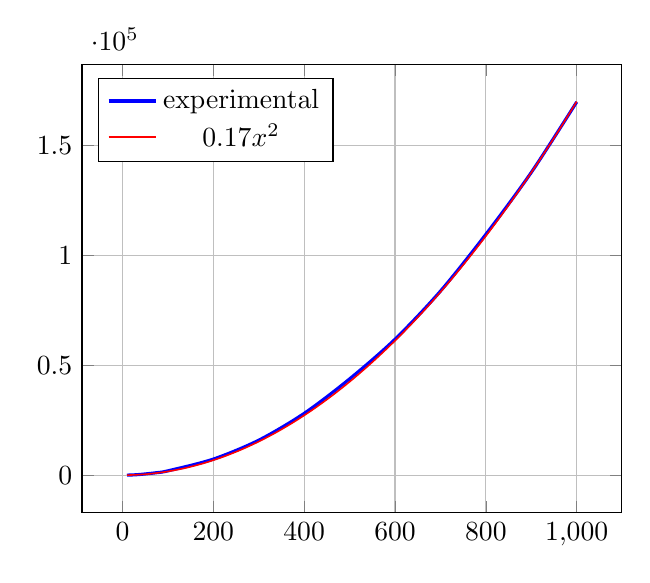
\begin{tikzpicture}
\begin{axis}[
    grid=major,
    legend pos=north west,
]
% Add your data points here
\addplot+[line width=0.4mm,smooth,mark=,error bars/.cd, y dir=both,y explicit ]
    coordinates {
        (10, 27)
        (20, 104)
        (30, 205)
        (40, 363)
        (50, 565)
        (75, 1139)
        (100, 1981)
        (200, 7323)
        (300, 15929)
        (400, 28127)
        (500, 43807)
        (600, 61860)
        (700, 83740)
        (800, 109585)
        (900, 137755)
        (1000, 169815)  
    };
\addlegendentryexpanded{experimental}
\addplot+[line width=0.2mm,smooth,mark=,domain=10:1000] {0.17*x^2};
\addlegendentryexpanded{$0.17x^2$}
\end{axis}
\end{tikzpicture}

Luke Tseng
\end{document}